En este capítulo se describe el diseño del sensor inteligente, explicando en detalle el hardware y software del mismo. En primer lugar se esbozan de forma general las actividades que debe llevar a cabo el sistema, luego se seleccionan los componentes necesarios para la implementación del prototipo de pruebas y finalmente se describen en detalle las actividades y los componentes que forman parte del sistema.

\section{Descripción breve del sistema}
\label{subsec:descpsist}

El sistema diseñado integra un conjunto de sensores y módulos que permiten medir variables dinámicas y cuasi-estáticas de un sistema estructural, enviarlas a larga distancia y posteriormente procesarlas y almacenarlas.

Una vez el sistema es encendido, ajusta de forma automática todos los sensores, eliminando el offset de los 3 ejes del acelerómetro y también del giróscopo utilizado para la estimación de inclinación. Además, se llevan a cabo comprobaciones de ``\textit{self test}'', que consiste en una prueba que verifica si el funcionamiento del sensor se encuentra dentro de los valores originales de fabricación, comparando con valores almacenados en registros internos del sensor. Una vez ajustado, el sistema envía de forma inalámbrica un mensaje a estación base para sincronizar la fecha y hora actual. El sistema ejecutará estas tareas de inicialización cada 2 registros de datos enviados con éxito.

Luego de la inicialización de los distintos módulos y el ajuste de la hora y fecha, el sistema comienza a medir de forma continua la aceleración triaxial, temperatura, humedad y estima la inclinación con sensores electrónicos de bajo consumo para posteriormente enviar los datos de forma inalámbrica a la estación base. Allí son recibidos, decodificados y pre-procesados para luego ser subidos vía inalámbrica a un computador que sirve de servidor en donde se almacenarán los datos, siendo controlado el sistema desde esta misma estación base, pudiendo enviar comandos de adquisición de datos de forma remota. A su vez, en la estación base se encuentra una interfaz gráfica que permite visualizar los datos obtenidos, realizar peticiones de datos a distancia, observar sus características principales, acceder al histórico de datos recogidos por el sensor, descargar los datos y ejecutar post-procesamiento a los mismos para evaluar las variables de interés para el monitoreo de salud estructural.

Puesto que la estación base está conectada a internet, el microcontrolador ubicado en la estación adquiere la fecha y hora actualizada utilizando un servidor del protocolo NTP (\textit{Network Time Protocol}) y sincroniza su RTC (\textit{Real Time Clock}) interno con estos valores. Una vez obtenida la fecha y hora, espera el comando de inicialización que envía de forma automática el sensor inteligente y ajusta el offset sus sensores, la cual le indica a la estación base que debe enviar la fecha y hora actual. De esta forma se sincronizan los relojes internos de ambos y permite al sensor inteligente tener la fecha y hora a la cual tomó el registro, enviando esta información como parte del registro de datos. La fecha y hora se envía bajo el formato \textit{UNIX Epoch}, el cual indica la cantidad de segundos transcurridos desde el 1 de Enero de 1970.
	
En la estación base, el sistema receptor se conectará a internet a través de la red WiFi, enviará los datos recibidos al computador en la estación base, siendo esta herramienta la encargada de pre-procesar los datos recibidos vía inalámbrica y convertirlos a un formato adecuado para poder ser almacenados en el computador y posteriormente procesados usando librerías de análisis numérico.

El comportamiento de los sistemas estructurales a estudiar condiciona los rangos e intervalos de medición de los sensores. La frecuencia de muestreo de la aceleración debe ser tal que al pasar del dominio del tiempo al dominio de la frecuencia, se obtenga un espectro que permita visualizar las componentes frecuenciales típicas para una estructura, las cuales suelen encontrarse por debajo de 100 Hz. Por su parte, la temperatura, humedad e inclinación suelen considerarse variables cuasi-estáticas, permitiendo que el sistema mida estas variables con intervalos lo suficientemente largos para poder monitorear cambios considerables en las mismas y posteriormente correlacionarlos a las condiciones estructurales. La frecuencia de muestreo de aceleración es deseable que esté limitada de tal forma que el espectro en frecuencia contenga las frecuencias de interés de la estructura.

El sistema en su funcionamiento normal está ejecutando las siguientes tareas principales:

\begin{itemize}
	\item Escuchando petición de trama de datos inmediata (Envía trama ante petición de estación base): Al recibir desde la estación base el comando de adquisición de datos, ejecutado desde la interfaz de control por el operador, el sistema comienza a tomar un registro de datos de forma inmediata, siempre y cuando el mismo no haya detectado previamente un evento importante que superara los límites establecidos, y lo envía a la estación base permitiendo que el usuario obtenga información del sistema en el instante en el cual se realiza la petición de los datos. Una vez es enviado y recibido con éxito la trama de datos, el sistema regresa a su estado anterior, tomando datos de forma continua y esperando alertas, comandos u horas programadas.
    \item Adquisición continua (envío programado a ciertas horas del día o ante eventos importantes): El sensor inteligente mide constantemente las variables de interés y envía periódicamente, a ciertas horas del día programadas con antelación, un registro de datos a la estación base. Al estar midiendo de forma continua, está atento a generar una interrupción o alerta ante algún valor de aceleración o inclinación que esté por encima de algún límite escogido con anterioridad que dependerá en gran medida de la estructura a monitorear y su naturaleza. Se escogió el valor de $2 \frac{m}{s^2}$ como generador de alerta, basado en la \textit{Escala de Mercalli} \citep{mercalli}, la cual indica que este valor de aceleración (que corresponde a 0.20 g) equivale a un sismo fuerte con daño moderado. El sistema envía de forma automática un registro de datos del acontecimiento importante que generó la alerta.

\end{itemize}

\section{Selección de componentes}
\label{sec:componentes}

Una vez definidas las tareas a realizar por parte del sistema, se procedió a escoger el hardware y los protocolos de comunicación para llevar a cabo el objetivo de diseñar un sensor inteligente para aplicaciones de monitoreo de salud estructural. 
	
\subsection{Protocolo de comunicaciones}

Para el protocolo de comunicación se buscaron protocolos capaces de manejar los datos recogidos por los sensores de forma eficaz y confiable. En este caso se refiere al protocolo utilizado para enviar los datos desde el sensor inteligente hasta la estación base. Sin embargo, se utilizaron distintos protocolos para la comunicación de los sensores con el microcontrolador y a su vez para comunicar la estación base con el receptor de datos.
	
Para el envío de datos a la estación base, preferiblemente el protocolo debía ser capaz de funcionar en rangos de distancia amplios, permitiendo que el sensor inteligente esté ubicado lejos de la estación base en donde serán monitoreadas las variables de interés. En primer lugar se escogieron algunos protocolos de forma preliminar, para luego estudiar a fondo sus características. Estos protocolos y sus características se resumen en la tabla \ref{tab:protocolos}:

\begin{table}[H]
    \centering
    \caption{Comparación entre protocolos de comunicación inalámbrica, \citep{IoTCompare} y \citep{LPWANCompare}}
    \label{tab:protocolos}
    \resizebox{\textwidth}{!}{%
    \begin{tabular}{|c|c|c|c|c|}
    \hline
    \textbf{Protocolo} & \textbf{Frecuencia} & \textbf{Rango} & \textbf{Velocidad} & \multicolumn{1}{l|}{\textbf{Consumo de energía}} \\ \hline
    \textbf{Zigbee} & 784 MHz/2.4 GHz & 100 m - 300 m & 250 kbps-500 kbps & Bajo \\ \hline
    \textbf{Sigfox} & 868 MHz/915 MHz & 3km - 10km & 100 bps & Bajo \\ \hline
    \textbf{NB-IoT} & LTE & 1km - 10km & 200 kbps & Bajo \\ \hline
    \textbf{WiFi} & 2.4 GHz/5.8 GHz & 100m & 54Mbps/1.3Gbps & Alto \\ \hline
    \textbf{Bluetooth} & 2.4 GHz & 10m - 100m & 720 kbps & Bajo \\ \hline
    \textbf{LoRa} & \begin{tabular}[c]{@{}c@{}}430 MHz/433 MHz\\ /868 MHz/915 MHz\end{tabular} & 15 km-30 km & 0.3kbs hasta 50 kbps & Bajo \\ \hline
    \end{tabular}%
    }
\end{table}


Con base en esta información, se escogió el protocolo LoRa como el más adecuado para el sensor inteligente, debido a su amplio rango y bajo consumo de energía. En general, la vasta mayoría de los módulos están basados en los chips fabricados por Semtech (los precursores del protocolo LoRa) SX126X y SX127X, por tanto se compararon ambas tecnologías en la tabla \ref{tab:moduloslora} para escoger el módulo más adecuado para el prototipo de pruebas a realizar:
% Please add the following required packages to your document preamble:
% \usepackage{graphicx}
\begin{table}[H]
    \centering
    \caption{Comparación entre módulos LoRa del fabricante Semtech \citep{datasheetSemtech}.}
    \label{tab:moduloslora}
    \resizebox{\textwidth}{!}{%
    \begin{tabular}{|c|c|c|c|c|c|}
    \hline
    \textbf{Módulo} & \textbf{Modem} & \textbf{Amplificador} & \textbf{Corriente RX} & \multicolumn{1}{l|}{\textbf{Sensibilidad}} & \textbf{Velocidad (bit rate)} \\ \hline
    \textbf{SX1261/62/68} & LoRa y FSK & \begin{tabular}[c]{@{}c@{}}+15 dBm - \\ +22 dBm\end{tabular} & 4.6 mA & -148 dBm & \begin{tabular}[c]{@{}c@{}}62.5 kbps \\ - 300 kbps\end{tabular} \\ \hline
    \textbf{S1272/73} & LoRa & +14 dBm & 10 mA & -137 dBm & 300 kbps \\ \hline
    \textbf{S1276/77/78/79} & LoRa & +14 dBm & 9.9 mA & -148 dBm & 300 kbps \\ \hline
    \end{tabular}%
    }
    \end{table}

\subsection{Sensores}

Para la selección de los sensores a utilizarse, es preciso definir las necesidades de un sistema de adquisición para sistemas estructurales, siendo su comportamiento el que define las características de los instrumentos de medición.

\subsubsection{Aceleración} 

En el caso de la medición de aceleración, el sensor inteligente debe contar con un sensor con las siguientes características:

\begin{itemize}
    \item Bajo nivel de ruido.
    \item Compensación de temperatura.
    \item Ancho de banda dentro del rango deseado en sistemas estructurales.
    \item Buena resolución.
    \item Suficientes grados de libertad.
    \item Compatibilidad con microcontroladores disponibles en el mercado.
    \item Bajo consumo
\end{itemize}

\subsubsection{Temperatura y humedad}

Para la medición de temperatura y humedad, el sensor inteligente debe contar con un sensor con las siguientes características:

\begin{itemize}
    \item Rango de trabajo dentro de las condiciones en las que se encuentre la estructura.
    \item Buena resolución y sensibilidad.
    \item Compatibilidad con microcontroladores.
    \item Bajo consumo.
\end{itemize}

\subsubsection{Inclinación}

Para la medición de inclinación, la cual, como se explica en la sección \ref{subsec:sensorfusion} el sensor inteligente debe contar con un sensor que cuente con las siguientes características:

\begin{itemize}
    \item Acelerómetro, giróscopo incorporado, convirtiéndose en una IMU (\textit{Inertial Measurement Unit}) o en el mejor de los casos,  incluir un magnetómetro, para convertirse en un MARG (\textit{Magnetic, Angular Rate, and Gravity})
    \item Bajo nivel de ruido.
    \item Buena resolución y sensibilidad.
    \item Compatibilidad con microcontroladores.
    \item Bajo consumo.
\end{itemize}

\subsection{Microcontroladores}

En el caso de los microcontroladores, se buscaron dispositivos capaces de obtener los datos provenientes de los sensores, procesarlos, almacenarlos temporalmente y posteriormente hacer uso del módulo de comunicaciones para su envío, usando este mismo módulo para recibir mensajes o comandos. También se tomaron en cuenta las capacidades de conexión inalámbrica de cada microcontrolador, su documentación y soporte por parte de los fabricantes, y por último su compatibilidad con los distintos frameworks, librerías y entornos de programación disponibles para los sensores y módulos, los cuales disminuyen el tiempo necesario para poner en marcha el funcionamiento del sistema. Se estudiaron las características de distintas placas de desarrollo, para posteriormente escoger la más adecuada. A continuación, en la tabla \ref{tab:microstabla}, se presentan las placas de desarrollo consideradas de forma preliminar y sus características principales:

% Please add the following required packages to your document preamble:
% \usepackage{graphicx}
\begin{table}[H]
    \centering
    \caption{Comparación entre placas de desarrollo basadas en MCU}
    \label{tab:microstabla}
    \resizebox{\textwidth}{!}{%
    \begin{tabular}{|c|c|c|c|c|c|c|}
    \hline
    \textbf{Placa} & \textbf{Procesador} & \textbf{Velocidad de reloj} & \textbf{RAM (kB)} & \multicolumn{1}{l|}{\textbf{ROM (kB)}} & \textbf{GPIO} & \textbf{Conectividad} \\ \hline
    \textbf{Teensy 4.0} & ARM M7 & 600 MHz & 1024 & 2048 & 40 & - \\ \hline
    \textbf{\begin{tabular}[c]{@{}c@{}}Raspberry Pi \\ Pico W\end{tabular}} & Dual ARM-M0 & 133 MHz & 264 & 2048 & 26 & WiFi \\ \hline
    \textbf{STM32 Discovery} & ARM M4 & 168 MHz & 192 & 1024 & 82 & - \\ \hline
    \textbf{STM32 Nucleo} & \begin{tabular}[c]{@{}c@{}}ARM M0 -\\ ARM M4\end{tabular} & \begin{tabular}[c]{@{}c@{}}84 MHz -\\ 180 MHz\end{tabular} & \begin{tabular}[c]{@{}c@{}}96 - \\ 128\end{tabular} & 512 & 50 & - \\ \hline
    \textbf{Espressif ESP32} & Dual Xtensa LX6 & 240 MHz & 520 & 4096 & 34 & WiFi/BT(BLE) \\ \hline
    \textbf{STM32 Blackpill} & ARM M4 & 100 MHz & 128 & 512 & 37 & - \\ \hline
    \end{tabular}%
    }
    \end{table}

\subsection{Diagramas de selección de componentes:}

\subsubsection{Selección del microcontrolador}

Siendo el componente central del sensor inteligente y el encargado de darle al sensor sus capacidades de interconexión y preprocesamiento, el microcontrolador cumple el rol más importante dentro del sistema. Para la elección de la placa de desarrollo a usar se tomaron en cuenta las placas estudiadas y mostradas en la tabla \ref{tab:microstabla} que mostraron potencial, obteniendo los resultados observados en la figura \ref{fig:arañamcu}

\begin{figure}[H]
    \centering
    \includegraphics[width = 0.9\textwidth]{imagenes/cap2_marcometod/ArañaMICROS.png}
    \caption{Diagrama de araña para selección de microcontrolador.}
    \label{fig:arañamcu}
\end{figure}

Con base en estos resultados, se escogió el microcontrolador ESP32 de Espressif Systems para ser el encargado de gestionar los datos provenientes de los sensores al ser el que se ajusta a las necesidades del proyecto para la construcción del prototipo de pruebas.

El  DevKit v1 es una placa de desarrollo creada por la empresa DOIT para evaluar el módulo ESP-WROOM-32. Esta permite acceder fácilmente a los pines del microcontrolador, además de proveer un puerto USB para la programación del mismo, incorporando un convertidor USB a serial en la tarjeta de desarrollo. También incorpora un regulador de voltaje que permite alimentar al microcontrolador con voltajes de hasta 12 V. En la figura \ref{fig:esp32} se observa la placa de desarrollo DevKit v1.

\begin{figure}[H]
    \centering
    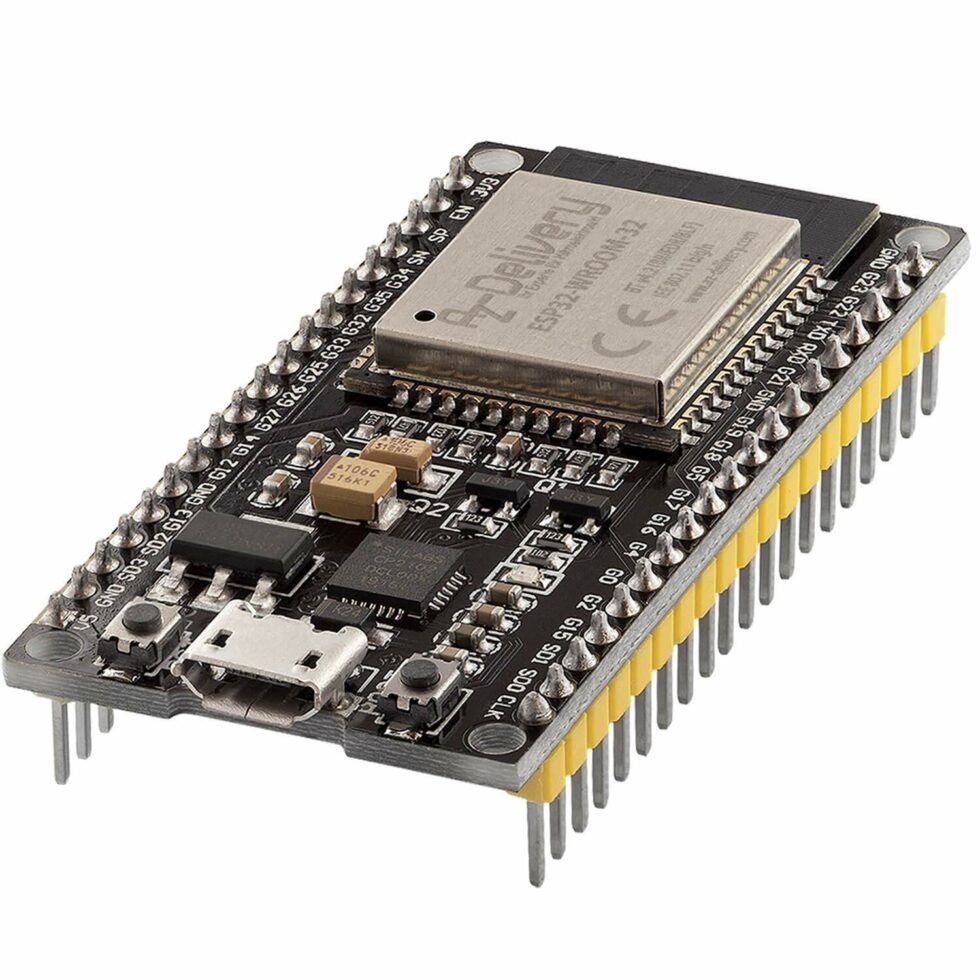
\includegraphics[width = 0.9\textwidth]{imagenes/cap2_marcometod/esp32.jpg}
    \caption{Placa de desarrollo ESP32 DevKit1 basada en el ESP32 de Espressif Systems.}
    \label{fig:esp32}
\end{figure}


\subsubsection{Selección del sensor de aceleración}

Con base en la información recopilada de distintos módulos de acelerómetros, se observa en la figura \ref{fig:arañaacl} que el MPU6050 de Invensense se ajusta a las necesidades del acelerómetro necesario para tomar los registros de vibración.

\begin{figure}[H]
    \centering
    \includegraphics[width = 0.7\textwidth]{imagenes/cap2_marcometod/ArañaACL.png}
    \caption{Diagrama de araña para selección de acelerómetro.}
    \label{fig:arañaacl}
\end{figure}

En la tabla \ref{tab:specs6050} se encuentran las especificaciones del módulo:

% Please add the following required packages to your document preamble:
% \usepackage{graphicx}
\begin{table}[H]
    \centering
    \caption{Especificaciones del MPU6050 de Invensense.}
    \label{tab:specs6050}
    \resizebox{\textwidth}{!}{%
    \begin{tabular}{|c|c|c|}
    \hline
    \textbf{Parámetro} & \textbf{Acelerómetro} & \textbf{Giróscopo} \\ \hline
    Rango a escala completa & $\pm2 g, \pm4 g, \pm8 g, \pm16 g,$ & $\pm250 ^\circ/s, \pm500 ^\circ/s, \pm1000 ^\circ/s, \pm2000 ^\circ/s$ \\ \hline
    Porcentaje de no linearidad & 0.5\% & 0.2\% \\ \hline
    Muestreo simultáneo & Sí & Sí \\ \hline
    Densidad espectral de potencia de ruido & $400 \mu g / / \sqrt{Hz}$ & $0.005 \mu ^\circ / \sqrt{Hz} $ \\ \hline
    Protocolo de comunicaciones & I2C & I2C \\ \hline
    Resolución del ADC & 16 bits & 16 bits \\ \hline
    Corriente & $500 \mu A$ & .6 mA \\ \hline
    \end{tabular}%
    }
    \end{table}

En la figura \ref{fig:mpu6050} se observa el módulo o \textit{breakout board} GY-521, el cual integra el acelerómetro MPU6050 y provee los pines necesarios para su integración en prototipos:

\begin{figure}[H]
    \centering
    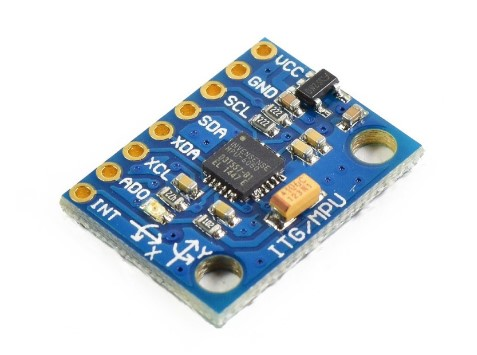
\includegraphics[width = 0.7\textwidth]{imagenes/cap2_marcometod/MPU6050BREAKOUT.jpg}
    \caption{Módulo GY-521 basado en el MPU6050 \citep{mpu6050}.}
    \label{fig:mpu6050}
\end{figure}


\subsubsection{Selección del sensor de temperatura y humedad}

Se observa en la figura \ref{fig:arañatemphum} que la mayoría de los sensores de temperatura y humedad, los cuales suelen estar integrados en un mismo módulo, no distan mucho en desempeño entre sí, sin embargo, entre ellos destaca el BME280 del reconocido fabricante Bosch, el cual cuenta con buena resolución además de una excelente documentación y librerías para distintos microcontroladores. El módulo SHT31 muestra potencial por su resolución. En este caso se descarta por la poca disponibilidad del módulo, pero es una buena opción para futuras implementaciones. Es por esta razón que se escogió el BME280 para llevar a cabo las mediciones de las variables ambientales en el prototipo de pruebas.

\begin{figure}[H]
    \centering
    \includegraphics[width = 0.9\textwidth]{imagenes/cap2_marcometod/ArañaTempHum.png}
    \caption{Diagrama de araña para selección de sensor de temperatura y humedad.}
    \label{fig:arañatemphum}
\end{figure}

En la tabla \ref{tab:specsBME280} se recopilaron las especificaciones más relevantes del sensor BME280:

% Please add the following required packages to your document preamble:
% \usepackage{graphicx}
\begin{table}[H]
    \centering
    \caption{Especificaciones del sensor BME280 de Bosch.}
    \label{tab:specsBME280}
    \resizebox{0.7\textwidth}{!}{%
    \begin{tabular}{|c|c|}
    \hline
    \textbf{Parámetro} & \textbf{Valor} \\ \hline
    Rango de humedad relativa & 0-100\% RH \\ \hline
    Precisión de humedad relativa & $\pm3 \%$ \\ \hline
    Rango de temperatura & $-40^\circ a 85^\circ $ \\ \hline
    Resolución de temperatura & $0.01 ^\circ$ \\ \hline
    Protocolo de comunicaciones & I2C \\ \hline
    Voltaje de operación & 1.8 V - 3.3 V DC \\ \hline
    Frecuencia de muestreo máxima & 157 Hz \\ \hline
    \end{tabular}%
    }
    \end{table}

El módulo GY-BME280 de la figura \ref{fig:bme280} permite acceder a los pines del sensor de forma sencilla, facilitando su integración en el prototipo de pruebas implementado:

\begin{figure}[H]
    \centering
    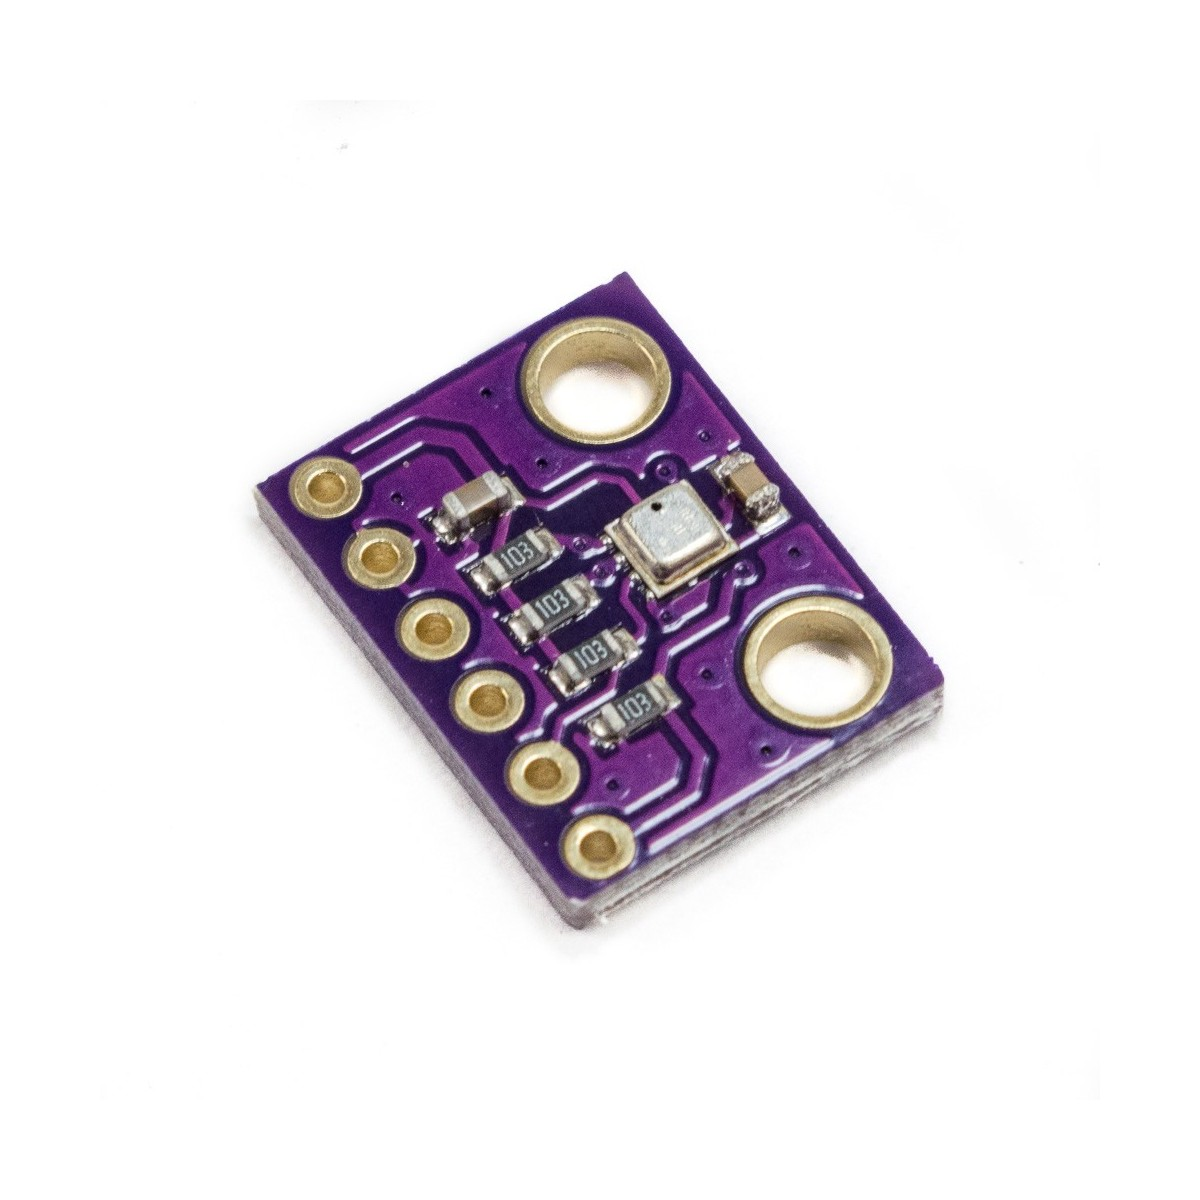
\includegraphics[width = 0.9\textwidth]{imagenes/cap2_marcometod/BME280BREAKOUT.jpeg}
    \caption{Módulo GY-BME280 basado en el sensor BME280 de Bosch \citep{bme280}.}
    \label{fig:bme280}
\end{figure}

\subsubsection{Selección del acelerómetro para estimación de ángulos}

Utilizando el mismo análisis que se llevó a cabo en la figura \ref{fig:arañaacl}, se modifica para fines de estimación de ángulo tomando en cuenta las premisas de la sección \ref{subsec:sensorfusion} para la fusión de sensores. Por tanto, con base en la figura \ref{fig:arañaimu} se escogió el módulo MPU9250, el cual cumple con la función de ser una MARG (\textit{Magnetic, Angular Rate, and Gravity}) de 9 grados de libertad, siendo ideal para la estimación de ángulos en el prototipo.

\begin{figure}[H]
    \centering
    \includegraphics[width = 0.7\textwidth]{imagenes/cap2_marcometod/ArañaIMU.png}
    \caption{Diagrama de araña para selección de unidad de medición inercial.}
    \label{fig:arañaimu}
\end{figure}


En la tabla \ref{tab:specs9250} se observan las características más relevantes del módulo:

% Please add the following required packages to your document preamble:
% \usepackage{graphicx}
\begin{table}[H]
    \centering
    \caption{Especificaciones del MPU9250 de Invensense.}
    \label{tab:specs9250}
    \resizebox{\textwidth}{!}{%
    \begin{tabular}{|c|c|c|c|}
    \hline
    \textbf{Parámetro} & \textbf{Acelerómetro} & \textbf{Giroscopio} & \multicolumn{1}{l|}{\textbf{Magnetómetro}} \\ \hline
    Rango a escala completa & $\pm2 g, \pm4 g, \pm8 g, \pm16 g,$ & $\pm250 ^\circ/s, \pm500 ^\circ/s, \pm1000 ^\circ/s, \pm2000 ^\circ/s$  & $\pm 4800 \mu T$ \\ \hline
    Porcentaje de no linearidad & 0.5\% & 0.1\% & - \\ \hline
    Muestreo simultáneo & Sí & Sí & No \\ \hline
    Densidad espectral de potencia de ruido & $300 \mu g / \sqrt{Hz}$ & $0.1 ^\circ/ \sqrt{Hz}$ & - \\ \hline
    Protocolo de comunicaciones & I2C/SPI & I2C/SPI & I2C/SPI \\ \hline
    Resolución del ADC & 16 bits & 16 bits & 14 bits \\ \hline
    Corriente & $450 \mu A$ & 3.2 mA & $280 \mu A$ \\ \hline
    \end{tabular}%
    }
    \end{table}

Similar al módulo GY-521, el módulo GY-9250 contiene al MPU9250 de Invensense y facilita el acceso a sus pines, además de incorporar un regulador de voltaje para poder alimentar el módulo con 5V. El módulo se observa en la figura \ref{fig:mpu9250}

\begin{figure}[H]
    \centering
    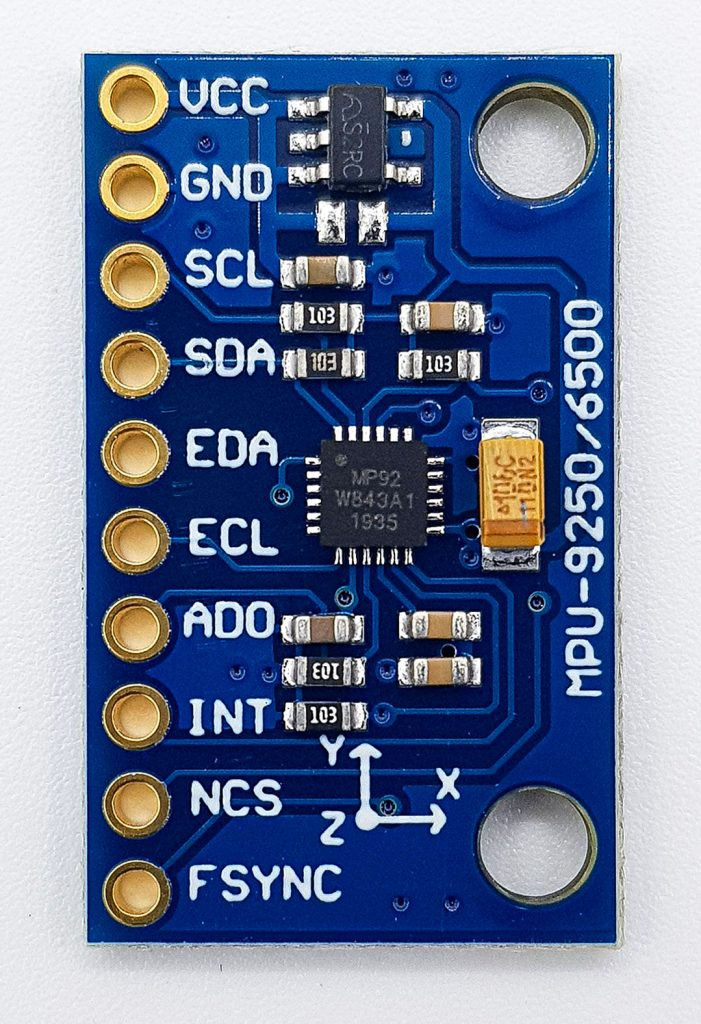
\includegraphics[width = 0.5\textwidth]{imagenes/cap2_marcometod/MPU9250.jpeg}
    \caption{Módulo GY-9250 basado en el MPU9250 de Invensense \citep{mpu9250}.}
    \label{fig:mpu9250}
\end{figure}


\subsubsection{Selección del módulo de comunicaciones}

Se ubicaron módulos de comunicaciones LoRa que fueran compatibles con el microcontrolador escogido, con documentación disponible y cuyas características se ajustaran a las necesidades del proyecto a llevar a cabo. Si bien el protocolo es el que condiciona las características de la gran mayoría de los módulos de comunicación del protocolo en cuestión, se buscó un módulo con facilidad de conexión e intercomunicación con el microcontrolador. Se observa en la figura \ref{fig:arañacomm} que la mayoría de los módulos tienen un desempeño similar, esto se debe a que están basados en distintas versiones de los módulos estudiados en la tabla \ref{tab:moduloslora}. Sin embargo, el condicionante es la disponibilidad y precio de los mismos, siendo el RA-02 de Ai-Thinker el seleccionado en este caso.

\begin{figure}[H]
    \centering
    \includegraphics[width = 0.7\textwidth]{imagenes/cap2_marcometod/ArañaTransmisores.png}
    \caption{Diagrama de araña para selección del módulo de comunicaciones.}
    \label{fig:arañacomm}
\end{figure}


\section{Detalle del diseño} A continuación se describe en detalle tanto el hardware como el software utilizado para llevar a cabo el sensor inteligente, además de las herramientas utilizadas para verificar su funcionamiento.


\subsection{Descripción detallada del sistema:}
\label{subsec:descripcion}

Complementando lo descrito en el apartado \ref{subsec:descpsist}, el prototipo del sistema se encarga de tomar registros de vibración estructural utilizando el acelerómetro MPU6050 mientras se miden variables ambientales, mediante el sensor de temperatura y humedad BM280, y se estima la inclinación mediante el módulo MARG MPU9250. Estos datos son recopilados y preprocesados por la tarjeta de desarrollo ESP32 DOIT DEVKIT, basada en el ESP32 de Espressif. Al encender el sensor inteligente, el cual será alimentado mediante el puerto USB-C de la tarjeta de desarollo o mediante una fuente de 5 V a los pines de alimentación del ESP32, este comienza la inicialización de los sensores con tareas que serán descritas con más detalle en apartados siguientes. Una vez culmina el ajuste inicial de los sensores, el sensor inteligente inicializa el módulo de comunicaciones LoRa RA-02 de Ai-Thinker, el cual una vez inicializado, envía un mensaje a la estación base solicitando la fecha y hora actual, con lo cual la estación base recibe, decodifica y responde al mensaje con los datos solicitados, lográndose la sincronización del reloj RTC interno del ESP32.

Luego de realizadas las tareas de inicialización y sincronización satisfactoriamente, el sensor inteligente comienza a tomar datos de todos los sensores de forma continua, manteniéndose alerta a cualquier evento que supere los valores límite en donde está ubicado el sensor. Como se describió en el apartado \ref{subsec:descpsist}, el sensor inteligente está configurado para enviar un registro ante los siguientes eventos:

\begin{itemize}
    \item El valor de aceleración medido por el sensor en algún eje supera el valor límite establecido.
    \item El reloj RTC interno indica que la hora actual se corresponde con una de las horas de envío programadas previamente.
    \item El sensor inteligente recibe un comando desde la estación base el cual indica que se comience a tomar un registro inmediato.
\end{itemize}

Una vez se toma el registro, este es almacenado temporalmente en buffers que son parte de estructuras de datos para posteriormente ser enviado utilizando el módulo de comunicaciones RA-02 de Ai-Thinker mediante paquetes sucesivos. Al terminar de enviar todos los paquetes, el sensor inteligente vuelve a su estado normal de toma de datos continua.

El sensor inteligente cuenta con 3 leds (\textit{Light Emitting Diodes}) indicativos:

\begin{itemize}
    \item LED Amarillo encendido: Ajuste e inicialización.
    \item LED Rojo intermitente: Toma de datos continua activa en espera de eventos.
    \item LED Verde encendido: Toma de un registro de datos por evento.
    
\end{itemize}

La tarjeta de desarrollo basada en el ESP32 utilizada cuenta con un LED azul integrado que se utiliza para notificar sobre la recepción o envío de algún paquete LoRa por el módulo de comunicaciones.

En la estación base se cuenta con otro módulo ESP32 DOIT DEVKIT, el cual se conecta a la red WiFi, dentro de la cual está ubicado un computador que cuenta con los servicios de NodeRED y Mosquitto, herramientas que se describirán en detalle más adelante. Este computador sirve de base de datos y broker para los datos a recibirse vía MQTT desde el ESP32 de la estación base, y además, proporciona una interfaz de monitoreo y control, basada en Python, la cual permite acceder a los registros y enviar comandos de adquisición de datos al sensor inteligente vía LoRa. 

Al estar conectado a WiFi, el ESP32 sincroniza su reloj RTC interno con el de un servidor del protocolo NTP. El ESP32 es el encargado de recibir los datos provenientes del sensor inteligente mediante un módulo de comunicaciones LoRa Ra-02 similar al del sensor inteligente. Los datos se almacenan temporalmente en buffers de datos para posteriormente convertirlos a formato JSON (\textit{JavaScript Object Notation}), el cual permite enviar los datos al broker MQTT en la red local. Una vez los datos son recibidos por el broker, estos son recibidos y procesados utilizando la herramienta NodeRED, la cual genera un formato tal que puede almacenarse en local usando el formato CSV (\textit{Comma separated values}). A su vez, NodeRED genera una notificación que envía un mensaje MQTT a la interfaz gráfica indicando que un nuevo registro está disponible. Los registros se guardan según su fecha y hora de llegada al broker en una carpeta específica en local.

La interfaz gráfica de usuario o GUI (\textit{Graphic User Interface}), basada en Python, se encarga de proporcionar una aplicación sencilla en donde pueden verse datos importantes de los registros, tales como:

\begin{itemize}
    \item Valores de inclinación de la estructura durante el registro escogido.
    \item Valores de temperatura y humedad del registro.
    \item Gráfico de aceleración vs. tiempo tomado por el sensor inteligente.
    \item Espectro en frecuencia utilizando la FFT del registro de aceleración.
    \item Valores máximos de picos en espectro en frecuencia (método de peak picking automatizado).
    \item Gráfico de la Densidad Espectral de Potencia (PSD por sus siglas en inglés).
    \item Gráfico de barras de los valores de inclinación para verificar si el dispositivo está a nivel.
\end{itemize}

Además de la posibilidad de visualizar y monitorear el estado de la estructura mediante la lectura de sus registros, la GUI permite:

\begin{itemize}
    \item Enviar un comando de adquisición de datos al sensor inteligente.
    \item Seleccionar el archivo a estudiar.
    \item Guardar el archivo seleccionado en otra ubicación, como puede ser un dispositivo extraíble o en una carpeta creada para un estudio en específico, en formato CSV.
    \item Indicación de registro nuevo disponible.
    \item Indicación de sensor inteligente a nivel, y de no estarlo, indica el eje en el que se debe ajustar.
    \item Fecha y hora del registro escogido para control de eventos.
    \item Botón de actualización de gráfica.
    \item Menú para escoger entre 3 funciones de aventanamiento distintas para ser aplicadas a los datos a procesarse.
\end{itemize}


\subsection{Diagrama general funcionamiento del sensor inteligente en conjunto con la estación base}

\begin{figure}[H]
    \centering
    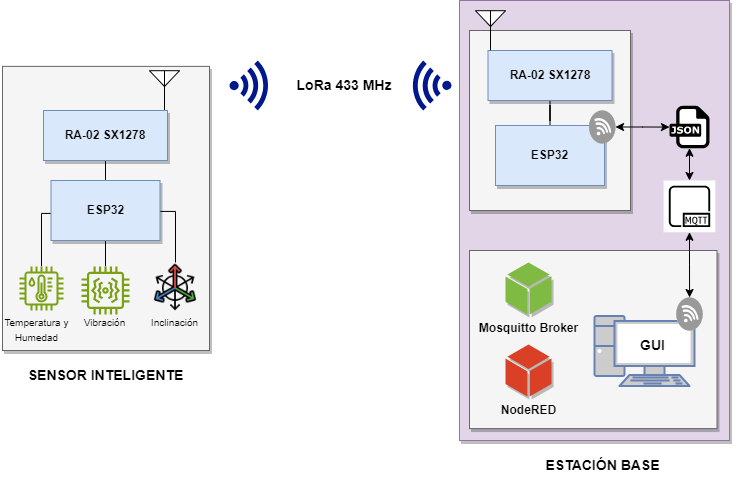
\includegraphics[width = \textwidth]{imagenes/cap2_marcometod/EsquemaGeneralSistema.png}
    \caption{Esquema general del sistema.}
    \label{fig:esquemageneral}
\end{figure}

\subsection{Descripción del hardware}

A continuación se describen las conexiones de hardware utilizando los componentes escogidos tanto para el sensor inteligente como para la estación base.

Basados en el funcionamiento del sistema explicado en el apartado \ref{subsec:descripcion} y \ref{subsec:descpsist}, y tomando en cuenta los componentes escogidos en el apartado \ref{sec:componentes}, se procede a realizar los siguientes diagramas de bloques de conexión: 

\subsubsection{Sensor inteligente:}

\begin{figure}[H]
    \centering
    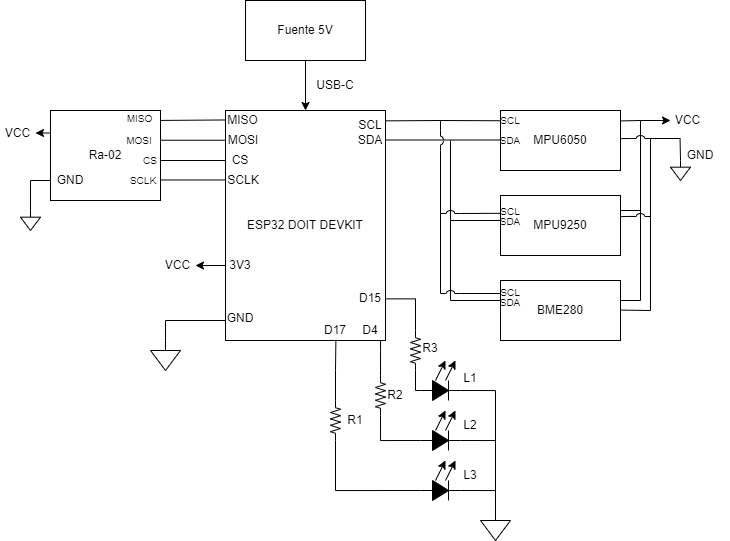
\includegraphics[width = 0.9\textwidth]{imagenes/cap2_marcometod/DiagramaHardwareSmartSensor.png}
    \caption{Diagrama de bloques del sensor inteligente.}
    \label{fig:smartsensorbloques}
\end{figure}

\subsubsection{Estación base:}

\begin{figure}[H]
    \centering
    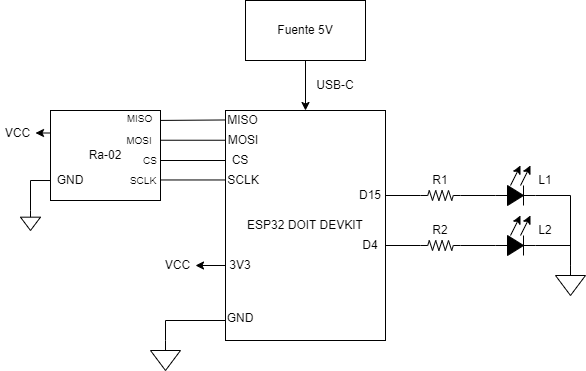
\includegraphics[width = 0.9\textwidth]{imagenes/cap2_marcometod/DiagramaHardwareEstacionBase.png}
    \caption{Diagrama de bloques de la estación base.}
    \label{fig:estacionbbloques}
\end{figure}

\subsection{Descripción del software}
\label{subsec:softwaredesc}

A continuación se describen las distintas tareas programadas tanto en el sensor inteligente como en la estación base para cumplir con el funcionamiento descrito en el apartado \ref{subsec:descripcion}.

\subsubsection{Programación del ESP32:} 

La documentación del fabricante del ESP32 \textit{Espressif Systems} especifica los requerimientos de hardware y software para poder programar el ESP32. En la figura \ref{fig:toolchain}, se observan las herramientas requeridas para subir un programa al microcontrolador. 

\begin{figure}[H]
    \centering
    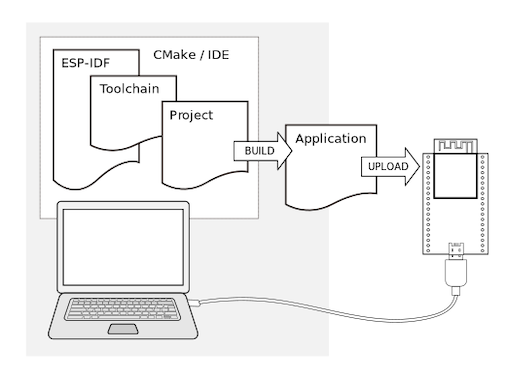
\includegraphics[width = 0.8\textwidth]{imagenes/cap2_marcometod/Toolchain.png}
    \caption{Ilustración del proceso para programar el ESP32 \citep{datasheetESP32}.}
    \label{fig:toolchain}
\end{figure}

PlatformIO surge como una necesidad de los desarrolladores de sistemas embebidos al tener que instalar herramientas específicas para cada fabricante de hardware, además de la tediosa tarea de la instalación de los toolchains y frameworks de trabajo para cada placa de desarrollo. El IDE (\textit{Integrated Development Environment}) de PlatformIO es una herramienta para sistemas embebidos que permite trabajar con múltiples plataformas, arquitecturas y frameworks en el mismo lugar, permitiendo programar distintos microcontroladores, acceder a librerías, e incluso depurar el código por línea dentro del mismo IDE. PlatformIO está disponible como una extensión del conocido IDE Visual Studio Code, desarrollado por Windows. Visual Studio Code es un editor de código ligero que permite crear aplicaciones en Windows y Linux.

Para el desarrollo del programa se utilizó PlatformIO v3.3.3 y Visual Studio Code en el sistema operativo Windows 10. El microcontrolador utilizado fue el ESP32 DOIT DevKit1, usando el Arduino Core del mismo. El Arduino Core permite programar el microcontrolador usando el lenguaje C++, además de las facilidades para la implementación de librerías por la gran comunidad que desarrolla proyectos usando esta herramienta.

\subsubsection{Librerías} 

Para llevar a cabo las distintas tareas del proyecto se hizo uso de una serie de librerías escritas en C++ para facilitar la comunicación con los sensores y módulos. A continuación se mencionan las librerías utilizadas y su función dentro del proyecto:

\begin{itemize}
    \item AdafruitBME280: Desarrollada por Adafruit, implementa rutinas para facilitar la comunicación con sensores Bosch BME280 de temperatura, humedad y presión, permitiendo acceder a los registros donde se almacenan las mediciones a través de la clase AdafruitBME280.
    \item AdafruitMPU6050: También desarrollada por Adafruit Industries, facilita la comunicación con sensores MPU6050, especialmente con placas de componentes o ``\textit{breakout boards}'', las cuales contienen el sensor y el hardware necesario para facilitar su comunicación y conexión a un microcontrolador a través de pines de salida. Implementa funciones de adquisición al leer los registros del sensor MPU6050. Para mejorar las capacidades de esta librería, se añadieron funciones de ``\textit{Self test}'' y de lectura de bytes tomadas de la implementación de Kris Winer de la librería MPU6050. La implementación de la clase AdafruitMPU6050 permite acceder a esta función de forma ordenada y sencilla.
    \item MPU9250: Desarrollada por Hideaki Tai. Se escogió por implementar algoritmos de estimación de inclinación basados en el filtro de Madgwick y Mahony. Se puede acceder a estas funciones a través de la clase MPU9250.
    \item RadioLib: Desarrollada por Jan Gromes, representa una de las librerías más utilizadas para comunicaciones inalámbricas en proyectos de sofware libre, soportando 13 módulos de comunicaciones distintos y 8 protocolos de comunicaciones distintos. Se escogió esta librería por su facilidad para controlar los módulos de Semtech de las serias SX126X y SX127X, permitiendo configurar el módulo, sus parámetros más importantes, y posteriormente implementar funciones propias basadas en interrupciones usando las funciones de la librería.
    \item ESP32Time y time: Desarrollada por Felix Biego, ESP32Time permite actualizar la estructura que contiene la fecha y hora actual del RTC interno del ESP32. A su vez, la librería ``time'', estándar de C, permite acceder a estos valores de fecha y hora. 
    \item PubSubClient: Desarrollada por Nick O'Leary, permite implementar la comunicación como cliente MQTT de forma sencilla en microcontroladores. Facilita la suscripción y publicación de datos a tópicos ubicados en un broker.
    \item ArduinoJson: Desarrollada por Benoit Blanchon, se complementa con la librería PubSubClient, permitiendo generar cadenas JSON para facilitar el envío de datos mediante MQTT.
\end{itemize}

\subsubsection{Programación de la aplicación de monitoreo y control}

Es conveniente contar con plataformas de monitoreo y control que sean de fácil acceso a los operadores del sistema para poder acceder a la información de la estructura de forma rápida y sencilla. 

Es común conseguir plataformas o aplicaciones propias de un fabricante. Estas suelen ser limitadas y, al ser propiedad del fabricante, usualmente no permiten ser personalizadas según la aplicación o caso de uso lo requiera.

Se buscaba implementar una aplicación sencilla que permitiera a los operadores acceder a los datos, almacenarlos en una ubicación deseada, que provea un formato de datos replicable y compatible con distintos programas, que permitiera acceder a los valores claves para el monitoreo de la salud estructural y que diera la posibilidad de modificarse según la aplicación lo requiera. Para esto, se diseñó una GUI utilizando Python en conjunto con la librería ``CustomTkinter''.

El programa, alojado en el computador y corriendo al estar el intérprete de Python instalado en el mismo, es capaz de enviar y recibir información vía MQTT usando la librería ``paho-mqtt''. Se implementó una interfaz gráfica de usuario utilizando ``customTkinter'' la cual provee distintos botones, widgets, menús y gráficas que permiten monitorear y controlar el sensor inteligente a distancia. 

A continuación se mencionan las librerías de Python 3.11.3 utilizadas en el programa para procesar y mostrar los gráficos una vez se accede a los archivos guardados en el computador, además del uso que se la da en la GUI:

\begin{itemize}
    \item CustomTkinter 5.2.2: Provee las herramientas para la creación de la GUI. Crea la ventana y subventanas, permite crear los distintos botones y menús, además de adjuntar gráficas y texto.
    \item Numpy 1.24.3: Permite ejecutar cálculos matemáticos y provee las funciones necesarias para llevar a cabo la FFT de los datos obtenidos del archivo leído. Permite manejar los arreglos de datos como matrices.
    \item Matplotlib 3.7.1: Es la responsable de graficar los datos de aceleración, inclinación, densidad espectral de potencia y el espectro en frecuencia a partir de arreglos de datos.
    \item Pandas 2.2.1: Permite acceder a los datos guardados como archivo CSV (``comma-separated-values'') y guardarlos para su posterior procesamiento.
    \item Scipy 1.11.1: Permite acceder a distintos tipos de filtro para pre-procesar los datos antes de ejecutar la FFT.
    \item Paho-mqtt 2.0.0: Provee las herramientas para crear un cliente MQTT capaz de suscribirse y publicar información a tópicos. Esta herramienta es la que permite recibir notificaciones sobre paquetes nuevos y enviar comandos al microcontrolador de la estación base para su posterior envío vía LoRa al sensor inteligente.
\end{itemize}



\subsubsection{Inicialización y setup}

Antes de comenzar con las rutinas de toma de datos, el sensor inteligente debe inicializar el hardware y eliminar el offset, además de la creación de tareas y colas. En primer lugar, las colas, encargadas de enviar información entre tareas como se describió en el apartado \ref{subsec:rtossubsec}, que fueron implementadas en el sensor inteligente son:

\begin{itemize}
    \item data\_temphumQueue
    \item aclQueue
    \item bufferQueue
    \item incQueue
    \item tramaLoRaQueue
    \item temphumarrayQueue
    \item incarrayQueue
\end{itemize}

Estas colas permiten que se envíe la información adquirida por una tarea, como puede ser obtener los valores leídos por el sensor mediante el objeto correspondiente a su clase, a otra tarea encargada de almacenarla en un buffer temporal para su posterior envío.

Una vez creadas las colas, se inicializa el hardware del sensor inteligente con las siguientes funciones:
\begin{itemize}
    
    \item bme.begin(): Inicializa el sensor BME280 usando el objeto bme. Dentro de esta rutina de la librería se definen los parámetros como modo de operación, cantidad de sobre muestreo en datos, duración del tiempo de standby.
    \item setup\_acl\_MPU6050(): Esta función inicializa el sensor MPU6050, configura su tiempo de muestreo a 200 Hz, enciende el led amarillo de ajuste, lleva a cabo la función de \textit{self test} y verifica que el valor se encuentre dentro de los valores nominales de fabricación. Posteriormente, se elimina el offset en todos los ejes al tomar 1000 mediciones y tomar el promedio de estas aceleraciones. Se inicializan los rangos del acelerómetro y se desactiva el filtro pasa-alto ya que, según la documentación del MPU6050 de Invensense, esto introduce retardo en las mediciones.
    \item setup\_mpu9250(): Esta función, análoga a las funciones anteriores, inicializa el MPU9250 usando el objeto creado perteneciente a la clase definida en la librería MPU9250. Se ejecuta una rutina de eliminación de offset similar a la del MPU6050 en donde se toman mediciones por un intervalo de tiempo, se promedian, y posteriormente se guardan en los registros de ``bias'' del dispositivo.
    \item setup\_lora\_radiolib(): La función de inicialización del módulo LoRa Ra-02 se encarga de configurar la frecuencia de trabajo, el factor de propagación y el ancho de banda. Luego de esto, envía un mensaje de inicialización en donde le hace saber al dispositivo de la estación base que el sensor inteligente ya se encuentra operativo y con sus sensores listos para las mediciones. Luego, se activa la interrupción (ISR por sus siglas en inglés), y se configura la función de \textit{callback} a ejecutar en caso de que la señal cambie de 0 V a un valor positivo en el pin 2 del microcontrolador. Esta ISR es la que permite manejar el caso en el que el módulo reciba una señal desde estación base. Una vez configurada la interrupción, se configura el módulo tal que escuche a mensajes presentes en el espectro.
    \item Wire.setClock(400000): Ajusta la frecuencia de las comunicaciones I2C del microcontrolador a 400 kHz.
\end{itemize}

En cuanto a la estación base, la inicialización consta de las siguientes funciones de configuración:

\begin{itemize}
    \item setup\_wifi(): Se encarga de conectarse a una red WiFi cuyas credenciales se encuentran definidas en un archivo wifi\_credentials.h. Si no logra conectarse, seguirá intentando hasta lograr la conexión a la red especificada.
    \item setup\_mqtt(): Si la conexión a la red WiFi es exitosa, el microcontrolador de la estación base se conecta al broker ubicado en la dirección IP especificada y asignada al computador donde está alojado el broker MQTT. Una vez ahí, se suscribe a un tópico al cual envía mensajes periódicos para que no se pierda la conexión. Finalmente, configura el tamaño del buffer del cliente a 40000 bytes.
    \item update\_timepacket(): Esta función tiene como objetivo actualizar el reloj RTC interno del ESP32 usando el protocolo NTP, con el cual el microcontrolador solicita a un servidor la fecha y hora actual, el servidor responde y esta información es almacenada en el ESP32.
\end{itemize}

Una vez configurado el hardware, se procedió a crear las tareas que se ejecutarán por el sensor inteligente. Para esto, se hace uso del comando xTaskCreatePinnedToCore de la siguiente forma:

\begin{lstlisting}[language=C++, caption=Creación de tareas en FreeRTOS]
    BaseType_t xTaskCreatePinnedToCore(TaskFunction_t pvTaskCode, const char * const pcName, const uint32_t usStackDepth, void * const pvParameters, UBaseType_t uxPriority, TaskHandle_t * const pvCreatedTask, const BaseType_t xCoreID);    
\end{lstlisting}

A todas las tareas se les asigna una prioridad, un \textit{handle}, el núcleo donde se ejecutarán y el espacio de memoria que pueden  ocupar dependiendo de la que necesite una vez se ejecute. 

\subsubsection{Estructuras de datos del sensor inteligente}

Se crearon distintas estructuras de datos para manejar las mediciones tomadas por los sensores y además permitir la comunicación entre tareas mediante colas, manteniendo los datos ordenados para posteriormente  enviarlos a larga distancia hacia y desde la estación base. Las estructuras más relevantes fueron:

\begin{itemize}
    \item BufferACL: Estructura que almacena los datos provenientes del sensor MPU6050 para enviarlos por paquetes utilizando el módulo de comunicaciones. Consta de 3 arreglos de 1024 flotantes cada uno.
    \item BufferTempHumedad: Almacena los valores de temperatura y humedad obtenidos por el sensor BME280. Estos valores son promediados previos al almacenamiento y además pasan por un filtro de primer orden que le asigna un mayor peso a la medición anterior para evitar cambios bruscos.
    \item BufferInclinacion: Almacena los valores de inclinación estimados por el sensor MPU9250 luego de implementar el Filtro de Madgwick.
    \item Packet: Corresponde a la estructura principal del sistema, ya que es la encargada de almacenar los distintos paquetes que surgen producto de la subdivisión del arreglo de flotantes de aceleraciones. Este paquete consta de los bytes de encabezado y el payload (los datos de aceleración adquiridos).
    \item Packet2: Sigue la estructura de Packet con la diferencia de tener un \textit{payload} de tamaño 1. Este paquete se corresponde con los mensajes de comandos desde y hacia estación base, los cuales constan de 1 solo byte.
    \item TimePacket: Se utiliza para actualizar el reloj RTC interno del ESP32 del sensor inteligente con la fecha y hora obtenida usando el protocolo NTP en la estación base.
    \item StringPacket: Es la encargada de almacenar el string de inicialización enviado por el sensor ingeligente una vez termina su inicialización y notifica a la estación base que está listo para actualizar su RTC y tomar datos.
    \item THIPacket: Siguiendo la estructura de los paquetes anteriores, esta estructura almacena los valores promedio de inclinación, temperatura y humedad que estaban almacenados en los buffers BufferInclinacion y BufferTempHumedad. Además, se incluye en esta estructura el timestamp correspondiente al momento en el cual se comienza a tomar el registro de datos de aceleración en formato ``\textit{UNIX Epoch}'', que corresponde al número de segundos transcurridos desde el 1 de enero de 1970, siendo este formato más sencillo de enviar y luego reconvertir en la estación base al formato de fecha y hora más adecuado.
\end{itemize}


\subsubsection{Programas del sensor ingeligente}

A continuación se describe el funcionamiento de las tareas y funciones para la adquisición y preprocesamiento de los datos:

\begin{itemize}
    \item Tarea de adquisición de datos de aceleración: Esta tarea es una de las más importantes del sensor inteligente. Se encarga de adquirir las mediciones de aceleración en los intervalos de tiempo especificados por el macro F\_SAMPLING. En esta tarea se verifica si los valores sobrepasan el límite de aceleración en alguno de los 3 ejes, también verifica si es hora de adquirir un registro según el reloj RTC interno del ESP32 y por último se asegura de que la bandera flag\_acl, la cual corresponde a una petición de datos vía LoRa desde la estación base, no se haya activado. En cualquiera de estos casos, la tarea envía los últimos 3 valores de aceleración registrados a una cola, la cual es recibida por una función que se encarga de almacenar estos valores en un buffer sucesivo hasta que se completan según el tamaño de registro fijado.
    
    \item Tarea de creación de buffer: Esta rutina es de gran importancia para el control y la sincronización de los eventos del sensor inteligente. Esto se debe a que es la encargada de evaluar si el buffer de datos ya fue llenado en su totalidad por los datos provenientes de la función de adquisición. De ser así, desactiva las tareas de adquisición temporalmente y activa la rutina de envío de datos por LoRa, la cual se encargará de reiniciar las tareas de adquisición. Además, reinicia todas las banderas límite para que el sensor inteligente esté alerta a nuevos eventos una vez se envíen todos los paquetes. 

    \item Evaluación de valores límite: La evaluación de los valores límite consiste en comparar los últimos valores de aceleración escogidos y levantar una bandera en caso de que alguno de los ejes sobrepase el límite de $2 [\frac{m}{s^2}]$.
    
    \item Verificación de hora actual: Esta función se encarga de verificar si la hora actual del microcontrolador, a la cual se puede acceder a través del objeto rtc de la librería ESP32Time, se corresponde con alguna de las horas previamente programadas en el sistema. De ser así, levanta una bandera para que el sensor inteligente comience a tomar un registro de datos.
    
    \item Tarea de adquisición de datos de temperatura y humedad: Esta tarea se encarga de adquirir los valores de temperatura y humedad del sensor BME280 y enviarlos mediante una cola a la función encargada de ejecutar los promedios y aplicar el filtro de primer orden a los datos para posteriormente llenar el buffer temporal de temperatura y humedad de forma sucesiva.

    \item Tarea de estimación de datos de inclinación: Análogo a las tareas de adquisición de aceleración, temperatura y humedad, esta tarea es la encargada de adquirir los valores de estimación de inclinación por parte del sensor MPU9250 para posteriormente, si se está tomando un registro de datos, enviar estos valores, usando una cola, a una función encargada de almacenar los valores promedio en un buffer temportal.

\end{itemize}

A continuación se describen las tareas encargadas de la comunicación de los datos vía LoRa en el sensor inteligente:



\begin{itemize}
    
    
    \item Rutina de interrupción: La rutina de interrupción o ISR es la encargada de reactivar la tarea de recepción de datos cuando en el pin asignado para la ISR se detecta un flanco ascendente. Estas rutinas se ejecutan en RAM por lo que requieren el macro ICACHE\_RAM\_ATTR específico para ESP32. Es decir, esta rutina siempre se ejecuta independientemente de la tarea que se esté ejecutando en el microcontrolador. Es importante acotar que se programó el sistema para desactivar esta interrupción mientras se está tomando un registro de datos. Esto impide que la recepción de un mensaje interrumpa la toma de los datos que ya está ejecutándose. A continuación, en el código \ref{code:ISRSS}, se observa la ISR implementada:
    
    \begin{lstlisting}[language=C++, caption=ISR de recepción de datos en sensor inteligente, label=code:ISRSS]
        void ICACHE_RAM_ATTR setFlag(void){  
            //Activo tarea de recepcion de datos
            vTaskResume(xHandle_receive_task);
            receivedFlag = true;
        }
    \end{lstlisting}

    La bandera de transmisión ``receivedFlag'' debe ser de tipo \textit{volatile}, para que pueda ser modificada dentro de una ISR.

    La interrupción se genera gracias a la configuración del módulo Ra-02 SX1278 de Ai-Thinker, el cual, al recibir un mensaje que cumpla con las características de encabezado de un mensaje LoRa, activa el pin DIO0 del módulo. Esta salida digital se conecta al pin configurado para detectar el flanco de subida y se genera la interrupción.
    
    \item Tarea de recepción de datos: Esta tarea es clave al ser la que decodifica la naturalez del mensaje recibido desde la estación base. Dependiendo de la longitud del mensaje recibido, se identifica si el mensaje corresponde a un comando de adquisición o a una actualización de RTC. Si la longitud no se corresponde con ninguno de los 2 casos, los datos está corrupta o no es para este receptor. Una vez se recibe el paquete con éxito, se verifica el payload y se levanta bandera de adquisición inmediata o se ejecuta función de actualización de RTC, según sea el caso.
    
    \item Tarea de envío de mensaje de inicialización: Es la encargada de enviar un string de inicialización a la estación base para notificar que el sensor inteligente ya culminó su período de inicialización y ajuste y está listo para una actualización de RTC.
    
    \item Función de actualización de RTC: Toma como entrada el arreglo de bytes recibido que contiene la informacion de la fecha y hora actual. La información se convierte a una estrucutra de datos de tipo TimePacket y se sincroniza el reloj interno del ESP32.
    
    \item Tarea de envío de paquetes de datos de aceleración: Una de las tareas de mayor importancia en todo el sistema al ser la encargada de gestionar el envío de los paquetes sucesivos de byte arrays a la estación base con la información almacenada en los buffers de aceleración correspondientes. 
    
    \item Función para generar arreglo de datos a enviar: Función para generar el arreglo de subpaquetes (chunks) que contienen 128 bytes cada uno para su posterior envío, mediante una cola, a la tarea de envio de datos LoRa en forma de byte array.
    
    \item Tarea de envío de datos de temperatura, humedad e inclinación: Una vez se envían todos los datos de aceleración, siguiendo la misma estructura de envío de datos de aceleración, se envían los contenidos del buffer promedio.
    
\end{itemize}


\subsubsection{Programas de la estación base:}

% Flujo de NodeRED de parseo de datos

\begin{itemize}
    
    \item Rutina de interrupción: Análoga a la ISR implementada en el sensor inteligente, se encarga de ejecutar en RAM la activación de la tarea encargada de la recepción de los datos independientemente del código que se esté ejecutando.
    
    \item Tarea de envío de fecha y hora para actualización de RTC: Esta tarea es la encargada de enviar una estructura de tiempo, dentro de una estructura de tipo TimePacket, al sensor inteligente con el fin de sincronizar su reloj RTC interno. Para el envío del paquete, se llena la estructura de tiempo y luego se convierte a un arreglo de bytes usando la línea de código presente en \ref{code:casting}, esto consiste en ``castea'' de un tipo de datos a otro. En este caso, es un cast de reinterpretación, permitiendo que esta conversión sea compatbile en distintas arquitecturas. La notación es originaria del lenguaje C y permite efectuar operaciones de bajo nivel con el puntero que contiene el byte array.
    
    \begin{lstlisting}[language=C++, caption=Conversión de datos a tipo byte array usando casting, label=code:casting]
        byte *byteArrTime = (byte *)&time_packet;
    \end{lstlisting}

    Una vez los datos están en el tipo byte array, el cual es aceptado por el módulo Ra-02 Ai-Thinker, los datos se envían utilizando el comando ``\textit{startTransmit}'' de la librería RadioLib. Este comando recibe como entradas el arreglo de datos de toda la estructura a enviar, la cual contiene el encabezado y el payload, y el tamaño del arreglo de datos final. Este comando devuelve un código de respuesta indicativo del estado del envío, notificando sobre si el envío fue exitoso o no.

    Una vez el arreglo de bytes es enviado con éxito, se debe introducir un retardo de 500 ms antes de configurar el módulo para que escuche comando nuevamente con el comando ``\textit{startReceive}'', como se observa en la figura \ref{code:loralisten}. La necesidad de este retardo surgió luego de observar que el módulo no recibía comandos si se configuraba para escuchar comandos inmediatamente después. Esto se debe a la necesidad del módulo de unos cuantos milisegundos para enviar el paquete exitosamente. Luego de enviar el paquete, se debe reiniciar la ISR para comenzar a escuchar paquetes nuevamente.

    \begin{lstlisting}[language=C++, caption=Configuración del módulo LoRa para escuchar paquetes, label=code:loralisten]
        int state2 = radio.startReceive();
        attachInterrupt(digitalPinToInterrupt(2), setFlag, RISING); // Reinicia ISR
    \end{lstlisting}
    
    \item Rutina para recepción de mensajes por MQTT: Para poder recibir mensajes vía MQTT, primero debe definirse la función callback a llamarse cuando se recibe un mensaje vía MQTT desde el tópico al cual está suscrito el microcontrolador.
    
    La función de callback está implementada como se observa en el código \ref{code:callbackmqtt}:

    \begin{lstlisting}[language=C++, caption=Función de callback para recepción de mensajes MQTT, label=code:callbackmqtt]
        void messageReceived(char* topic, byte* payload, unsigned int length) {

            //Convierte payload a string
            String mensaje;
            for (int i = 0; i < length; i++) {
                mensaje += (char)payload[i];
            }

            //Chequear si el mensaje recibido es "ON"
            if (message == "ON") {
                //Llama a la ISR, peticion de datos al Smart Sensor
                if(!transmitFlag){
                    ISR_MQTT_Request(); //ISR
                }
            }
        }
    \end{lstlisting}
    
    \item Tarea de envío de comandos de adquisición al sensor inteligente:
    
    Una vez se recibe vía MQTT el comando, ejecutado desde la GUI por el operador, de enviar un comando de adquisición de datos al sensor inteligente, se ejecuta la ISR, que se implementó como se observa en el código \ref{code:isrcomando} que activa la envío de datos usando el módulo LoRa:

    \begin{lstlisting}[language=C++, caption=ISR de activación de envío de comando por LoRa, label=code:isrcomando]
    //Rutina de ISR por software en caso de recibir una peticion por MQTT
    void IRAM_ATTR ISR_MQTT_Request()
    {
        transmitFlag = true;
        vTaskResume(xHandle_send_task);
    }
    \end{lstlisting}

    La tarea de envío de datos por LoRa, se encarga de enviar en el payload el byte 0x01, este payload es decodificado e identificado por el sensor inteligente y lo interpreta como un comando, activando la toma de datos.

    Los comandos utilizados son análogos a los utilizados en el envío de datos para la actualización del RTC, definida anteriormente. Podrían numerarse de la siguiente forma:

    \begin{enumerate}
        \item Desactivar interrupción.
        \item Llenar la estructura de datos a enviar.
        \item Convertir la estructura de datos al tipo de datos byte array para su envío.
        \item Enviar el paquete LoRa usando el comando ``startTransmit'' de la librería RadioLib.
        \item Introducir retardo de 500 ms para que el módulo pueda enviar con éxito el paquete.
        \item Reiniciar bandera de transmisión.
        \item Configurar el módulo a modo ``\textit{listening}''.
        \item Reactivar interrupción.
    \end{enumerate}

    \item Tarea de recepción de datos provenientes del sensor ingeligente: Corresponde a la tarea principal de la estación base. Se encarga de recibir y almacenar los datos recibidos vía LoRa para su posterior subida al broker MQTT. 
    
    Para lograr esto, la tarea lleva a cabo los siguientes pasos:

    \begin{enumerate}
        \item Reinicia bandera de ISR.
        \item Crea unión packetUnion para que contenga las distintas estructuras que pueden utilizarse.
        \item Lee los datos recibidos y obtiene el tamaño del paquete.
        \item Dependiendo del tamaño del paquete se activan distintas banderas que identifican el mensaje como datos de aceleración, datos de temperatura y humedad o un mensaje de inicialización del sensor inteligente.
            \begin{itemize}
                \item Caso 0 (Datos de aceleración): Se guardan los arreglos de datos en buffers sucesivos, los cuales se identifican dependiendo de la identificación presente en el encabezado del mensaje. El número de paquetes está fijado por el número de bytes que se envían en cada payload. Una vez se reciben todos los paquetes, se envían los buffers en una cola para su posterior envío vía MQTT.
                \item Caso 1 (Mensaje de inicialización de sensor inteligente): Al recibir un mensaje de inicialización del sensor inteligente, esto significa que el sensor culminó su proceso de ajuste e inicialización y está listo para sincronizar su RTC. En este caso, se identifica el messageID del mensaje y si cumple con las características de la inicialización del RTC, se envía el mensaje correspondiente.
                \item Caso 2 (Datos de temperatura y humedad): Análogo al caso 0, si se identifica el mensaje como uno que corresponde a datos de temperatura y humedad a partir de se almacenan los datos de temperatura humedad e inclinación en una estructura dedicada. Esta se envía mediante una cola a la tarea encargada de subir los datos al broker MQTT.
            \end{itemize} 
        \item En caso de tratarse de datos corruptos cuya CRC no corresponda con la esperada por el receptor, se descartan.
    \end{enumerate}
        
    \item Tarea de envío de datos de temperatura, humedad e inclinación al broker vía MQTT:
    
    Esta tarea tiene como objetivo subir los datos recibidos mediante una cola, enviada por el RTOS luego de recibir los datos de temperatura, humedad e inclinación, al broker ubicado en el computador cuya dirección IP es conocida. Para lograrlo se llevaron a cabo los siguientes pasos:

    \begin{enumerate}
        \item Suspende temporalmente la tarea \textit{keepalive\_task}, encargada de enviar mensajes cortos de forma periódica al broker y mantener activa la conexión mientras no se están enviando datos.
        \item Crea estructura de datos de tipo THIPacket.
        \item Recibe la cola con los datos.
        \item Ejecuta la función \textit{sendTHI}, la cual recibe como entrada el tópico y el dato a enviar. Esta función convierte los datos a tipo string y luego los publica en el tópico de interés.
        \item Activa la tarea para envío de datos de aceleración
        \item Se suspende a sí misma.
    \end{enumerate}
    
    \item Tarea de envío de arreglos de datos de aceleración al broker vía MQTT:
    
    Similar a la tarea anterior, se encarga de subir los datos de aceleración recibidos mediante una cola al broker MQTT. Se llevaron a cabo los siguientes pasos para subir exitosamente los datos:

    \begin{enumerate}
        \item Recibe la cola con los arreglos de aceleración y los almacena en una estructura de datos.
        \item Ejecuta la función ``\textit{sendAxis}'', similar a ``\textit{sendTHI}'', la cual recibe como entrada el tópico, el nombre del eje que está siendo enviado, el arreglo de datos almacenado en la estructura y el tamaño del arreglo. Esta función crea un ``nestedArray'', es decir, crea nuevo array JSON anidado. El arreglo se llena con los datos de forma sucesiva utilizando un bucle. Luego, serializa el documento JSON a una cadena de texto. Finalmente, la representación en texto del documento JSON es publicada al tópico de interés.
        \item Reinicia la ejecución de la tarea \textit{keepalive\_task}.
        \item Se suspende a sí misma hasta que sea reanudada en el próximo envío.
    \end{enumerate}
    
\end{itemize}

\subsubsection{Aplicación de monitoreo y control:}

A continuación se describen las funciones del sistema de monitoreo y control:

\begin{itemize}
    
    \item Conexión MQTT: La aplicación se conecta al broker MQTT ubicado en la dirección IP del computador. Para lograrlo, se ejecuta la función \textit{connect} de la librería paho-mqtt, la cual recibe como entradas la dirección IP del broker, el puerto de conexión y el nombre del cliente. Una vez conectado, se suscribe y publica a los tópicos de interés.
    
    \item Petición de datos a sensor inteligente: La aplicación permite al operador solicitar datos al sensor inteligente mediante el envío de un mensaje vía MQTT al tópico encargado de gestionar el envío de comandos al sensor inteligente. Para lograrlo, se ejecuta la función \textit{publish} de la librería paho-mqtt, la cual recibe como entradas el tópico de interés y el mensaje a enviar.
    
        
    \item Gráfica de aceleración en tiempo: Para las gráficas se hizo uso de la librería matplotliob, la cual proporciona las herramientas necesarias para mostrar gráficamente series de datos que pueden estar almacenados en arreglos. En el caso de la aceleración, se lee el registro escogido por el operador en formato ``csv'' y se almacenan las columnas correspondientes en arreglos de la librería ``NumPy''. El eje x, que representa el tiempo, se construye a partir de la frecuencia de muestreo y el número de muestras. Luego, se grafican los datos en función del tiempo.
    
    \item Gráfica de espectro en frecuencia: Ejecutando la FFT sobre los datos de aceleración almacenados en arreglos de NumPy, se obtiene el espectro en frecuencia del registro escogido. El eje x debe truncarse para graficar solo las frecuencias positivas. Se incluyen en la gráfica indicadores que apuntan a los valores máximos por eje.
    
    \item Valores de temperatura, humedad e inclinación: En el archivo escogido por el operador se encuentran los valores de las variables ambientales y la inclinación en columnas separadas. Estos datos se almacenan y se agregan a la ventana. 
    
    \item Gráfica de barras para inclinación: Los valores de inclinación utilizados para ser mostrados en la ventana, se usan para construir un gráfico de barras que permite al operador saber si el sensor inteligente se encuentra a nivel en un rango dado. Además, en caso de no estar dentro del rango deseado, se notifica sobre el ángulo que debe ajustarse para que el sensor inteligente esté a nivel.
    
    \item Gráfica de Densidad Espectral de Potencia: Similar al proceso para obtener la gráfica del espectro en frecuencia, se ejecuta la densidad espectral de potencia elevando al cuadrado los arreglos que contienen los espectros, graficando posteriormente estos valores contra el número de datos obtenidos en frecuencia.
\end{itemize}

% \subsection{Diagrama de flujo del sistema}


% \subsection{Diagrama de funcionamiento del sistema}
